\documentclass{jsarticle}
\usepackage[dvipdfmx,hiresbb]{graphicx}
\usepackage{amsmath,amssymb}

\begin{document}
\title{包絡線定理}
\author{鈴木花奈子}
\maketitle

\section{包絡線定理}

包絡線定理とは、パラメータつきの最大化問題である、

\[ v(\alpha)=\max_{x} f(x,a) , x\in \mathbb{R}^n , \alpha \in \mathbb{R}^m\]

を考える。

\begin{enumerate}
\item どういうときに$v$は微分可能か
\item 微分可能な時に$\frac{\partial v}{\partial\alpha_{j}}$はどう書けるか
\end{enumerate}
の答えを考えたい。

微分可能性を仮定して、$\frac{\partial v}{\partial\alpha_{j}}$を求めた際に、
\begin{enumerate}
\item 最適解を代入してからパラメータで微分したもの
\item パラメータ微分してから最適解を代入したもの
\end{enumerate}
の二つが等しくなることを、\textgt{\large 包絡線定理}と呼ぶ。
           

また、$f(x,\alpha)$を、$\alpha-\beta$平面において、曲線
\[ l_{x}: \beta=f(\alpha)\]
とみたとき、曲線$\beta=v(\alpha)$は直線群$l_{x}$の\textgt{\large 包絡線}であるという。

\pagebreak
\section{コードについて}
\subsection{コード}
今回私が包絡線定理のために書いたコードは以下の通りです。

                      

1~~~\# -*- coding: utf-8 -*-

2~~~import matplotlib.pyplot as plt

3~~~from mpl\_toolkits.axes\_grid.axislines import SubplotZero

4~~~import numpy as np

5~~~import fractions

6~~~FIGNUM = 1 

7~~~if FIGNUM == 0:

8~~~~~~$t\_max, step = 2, fractions.Fraction(1,3)$
    
9~~~if FIGNUM == 1:

10~~~~~$t\_max, step = 3, fractions.Fraction(1,2)$

11~~$x\_max = 7$

12~~$y\_max = 6$

13~~$y\_min = -5$

14~~def f(x, t):

15~~~~~~return $t*x-t**2$

16~~$t\_min = -t\_max$

17~~$x\_min = -x\_max$

18~~if 1:

19~~~~~~$fig = plt.figure(1)$
    
20~~~~~~$ax = SubplotZero(fig, 111)$
    
21~~~~~~$fig.add\_subplot(ax)$

22~~~~~~for direction in ["xzero", "yzero"]:
    
23~~~~~~~~~~ax.axis[direction].set\_axisline\_style(``$-{\mid}>$'')
        
24~~~~~~~~~~ax.axis[direction].set\_visible(True)

25~~~~~~for direction in ["left", "right", "bottom", "top"]:
    
26~~~~~~~~~~ax.axis[direction].set\_visible(False)

27~~~~~~ax.text(0, y\_max, 'y')
    
28~~~~~~ax.text(x\_max, 0, 'x')
    
29~~~~~~plt.xticks([])
    
30~~~~~~plt.yticks([])
    
31~~~~~~plt.xlim(x\_min, x\_max)
    
32~~~~~~plt.ylim(y\_min, y\_max)

33~~~~~~$x = np.linspace(x\_min, x\_max, 100)$

34~~~~~~for t in np.arange(t\_min, t\_max+step, step):
    
35~~~~~~~~~~$y = f(x, t)$

36~~~~~~~~~~ax.plot(x, y, color='black', linewidth=1)

37~~plt.savefig('envelope'+str(FIGNUM)+'.png')

38~~plt.savefig('envelope'+str(FIGNUM)+'.pdf')

39~~plt.show()

\subsection{コードの説明}
\begin{itemize}
\item 今回は、2種類の直線群それぞれについて包絡線を描くとを目指した。
そこで、6~10行目では6行目の値を0か1に変更させることで好きな方の図を表示させられるようにした。
\item 16~17行目では対称性を利用して変数を設定できるようにし、入力の手間が省けるようにした。
\item 34~36行目では、パラメータの上限と下限、およびその間いくつ刻みで直線群を描くかをarange関数を利用して設定し、for文によって繰り返しを行った。
\item 軸のデザインが少し見栄えがよくないままであったり、いただいたヒントをそのまま適用しただけの部分が多いため、今後は自在に操れるようにさらに学習を重ねていきたい。
\end{itemize}

\subsection{実行結果}
\[ f(t,x)=-t^2+xt \]とし、パラメータ$t$の上限および下限、いくつ刻みかを変化させた結果、以下の2つの図を得ることができた。
\begin{figure}[h]
	\centering
	\begin{minipage}{0.4\columnwidth}
		\centering
		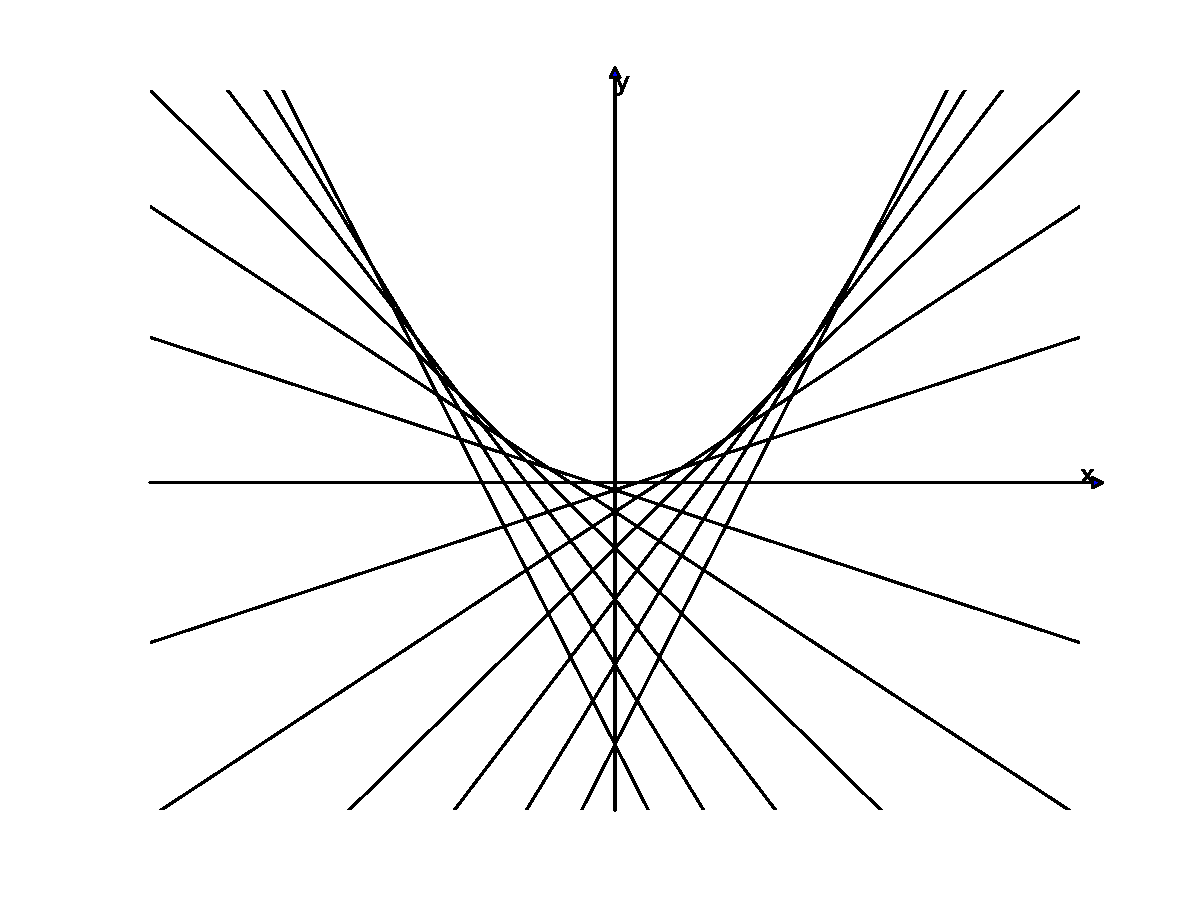
\includegraphics[width=7cm]{envelope0.pdf}
		\caption{傾き-2~2、1/3刻みのグラフ}
		\label{fig0}
	\end{minipage}
	\begin{minipage}{0.4\columnwidth}
		\centering
		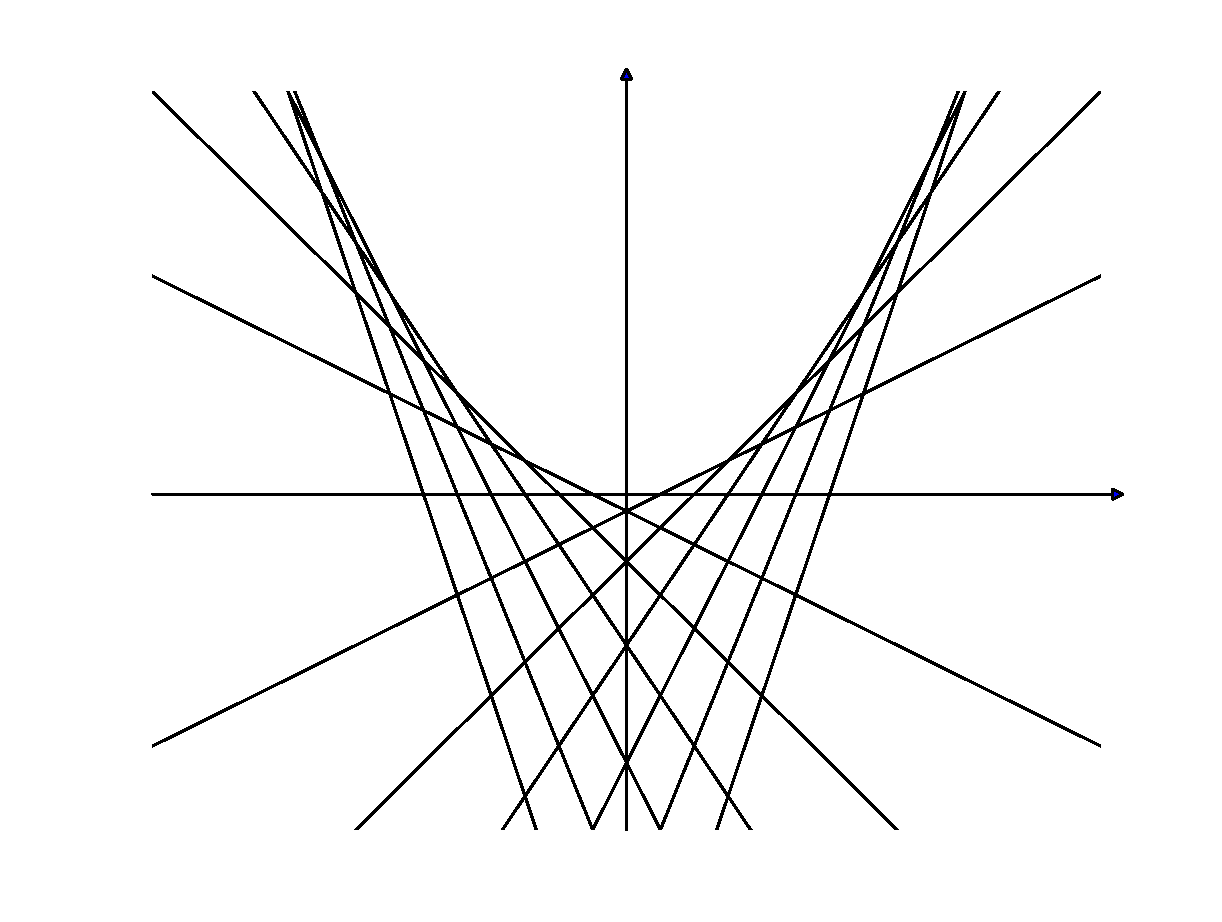
\includegraphics[width=7cm]{envelope1.pdf}
		\caption{傾き-3~3、1/2刻みのグラフ}
		\label{fig1}
	\end{minipage}
\end{figure}%/

\begin{thebibliography}{9}
\item 2013年度「経済学のための数学」講義ノート
\item 尾山大輔、安田洋祐「経済学で出る包絡線定理」『経済セミナー』2011年10/11月. pp. 38-39. 日本評論社
\end{thebibliography}

\end{document}
